\section{Literature review}

\subsection{Mathematical models}

\begin{frame}{Compartmental models}
    \begin{block}{\gls{SEIR} model \cite{brauerCompartmentalModelsEpidemiology2008}}
        \begin{equation*}
            \begin{aligned}
                S' &= - \beta(N)SI \\
                E' &= \beta(N)SI - \kappa E \\
                I' &= \kappa E - \alpha I \\
                R' &= f \alpha I \\
                N' &= - (1 - f) \alpha I
            \end{aligned}
        \end{equation*}
    \end{block}

    \begin{figure}
        \centering
        \begin{tikzpicture}[->, > = stealth', node distance = 2cm, thick]
            \node[state]               (S) {S};
            \node[state, right of = S] (E) {E};
            \node[state, right of = E] (I) {I};
            \node[state, right of = I] (R) {R};
            \draw (S) edge node[above]{$\beta$}  (E)
                (E) edge node[above]{$\kappa$} (I)
                (I) edge node[above]{$\alpha$} (R);
        \end{tikzpicture}
        \caption{States graph for the \gls{SEIR} model}
        \label{fig:seir-model-transition-graph}
    \end{figure}
\end{frame}

\begin{frame}{Agent-based models}
    \begin{figure}[!htb]
        \centering
        \subcaptionbox{Transmission networks}{
            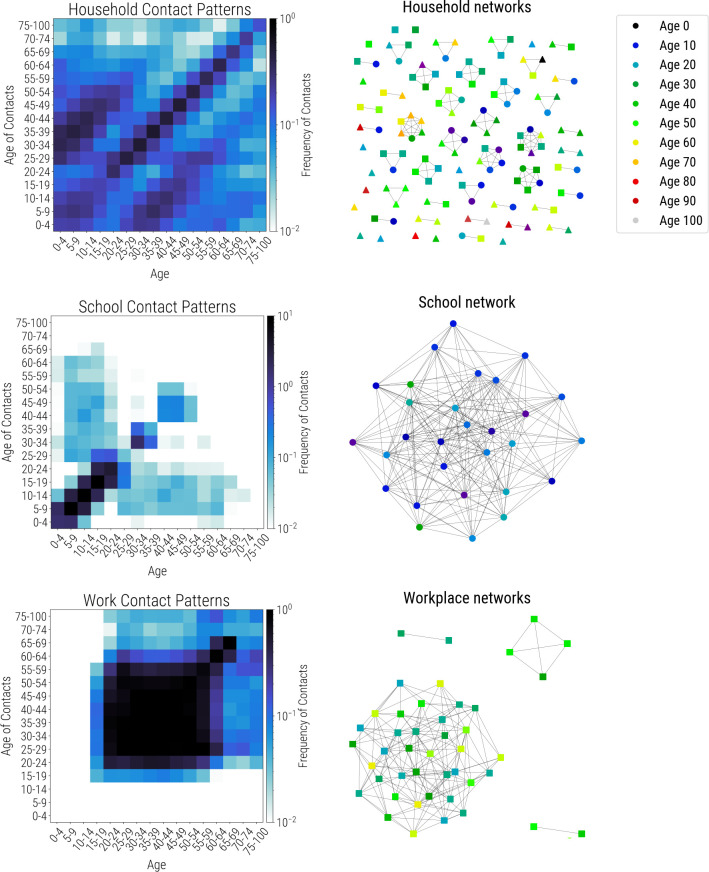
\includegraphics[scale=0.7]{covasim-networks.jpg}
        }
        \subcaptionbox{States graph}{
            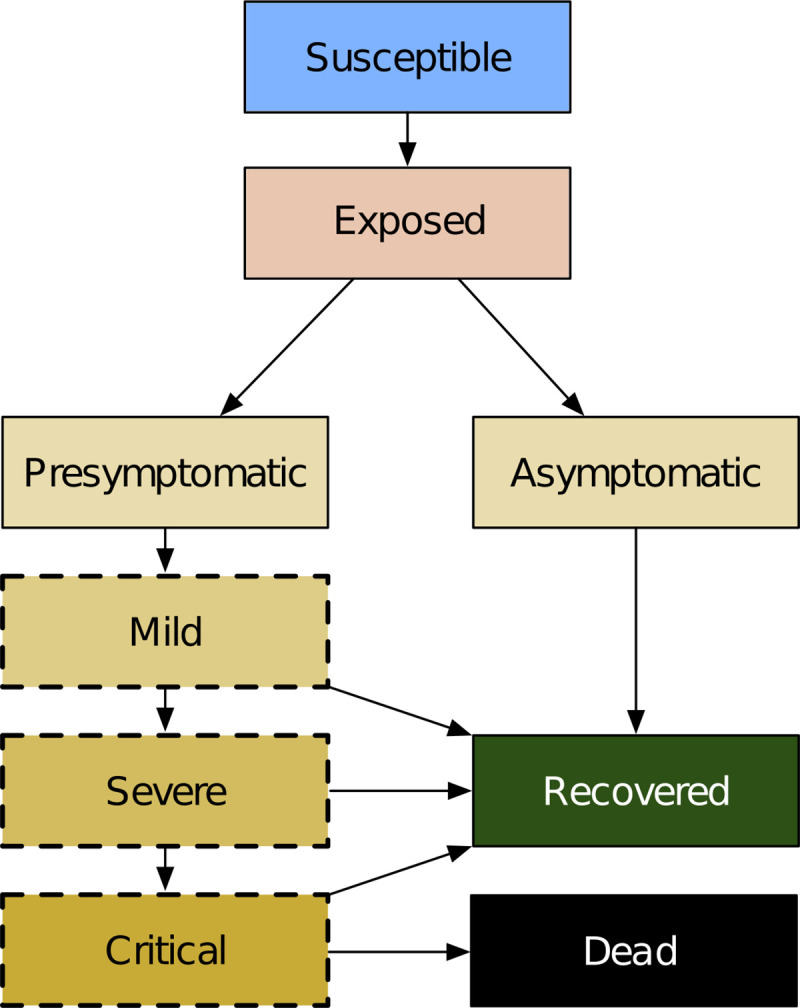
\includegraphics[scale=0.5]{covasim-compartments.jpg}
        }
        \caption{Covasim model \cite{kerrCovasimAgentbasedModel2021}}
        \label{fig:covasim-schematics}
    \end{figure}
\end{frame}

\begin{frame}{Pros \& cons}
    \begin{exampleblock}<1->{Pros}
    \begin{itemize}
        \item Explainable
        \item Based on many years of research
        \item Easy to understand and implement
    \end{itemize}
    \end{exampleblock}

    \begin{alertblock}<2->{Cons}
    \begin{itemize}
        \item Low representational capabilities
        \item The represented dynamics are stationary
        \item Unrealistic assumptions about real-world scenarios
    \end{itemize}
    \end{alertblock}
\end{frame}

\subsection{Data-driven models}

\begin{frame}{Examples}
    \begin{itemize}
        \item<1-> \glsfirst{ARIMA} models \cite{ceylanEstimationCOVID19Prevalence2020,singhPredictionCOVID19Pandemic2020,ribeiroShorttermForecastingCOVID192020}
        \item<2-> Explainable \glsfirst{ANN} encoder \cite{ramchandaniDeepCOVIDNetInterpretableDeep2020}
        \item<3-> \glsfirst{RNN} \cite{chimmulaTimeSeriesForecasting2020,shahidPredictionsCOVID19Deep2020}
        \begin{itemize}
            \item \glsfirst{LSTM}
            \item \glsfirst{Bi-LSTM}
            \item \glsfirst{GRU}
        \end{itemize}
    \end{itemize}
\end{frame}

\begin{frame}{Pros \& cons}
    \begin{exampleblock}<1->{Pros}
    \begin{itemize}
        \item High prediction accuracy
        \item Allow for modeling without needing domain knowledge
    \end{itemize}
    \end{exampleblock}

    \begin{alertblock}<2->{Cons}
    \begin{itemize}
        \item Unexplainable
        \item Relied on large amount of data
        \item Inability to capture the true disease dynamics
    \end{itemize}
    \end{alertblock}
\end{frame}

\subsection{Novel compartmental models}

\begin{frame}{Incorporating mobility data}
    \begin{figure}[!htb]
        \centering
        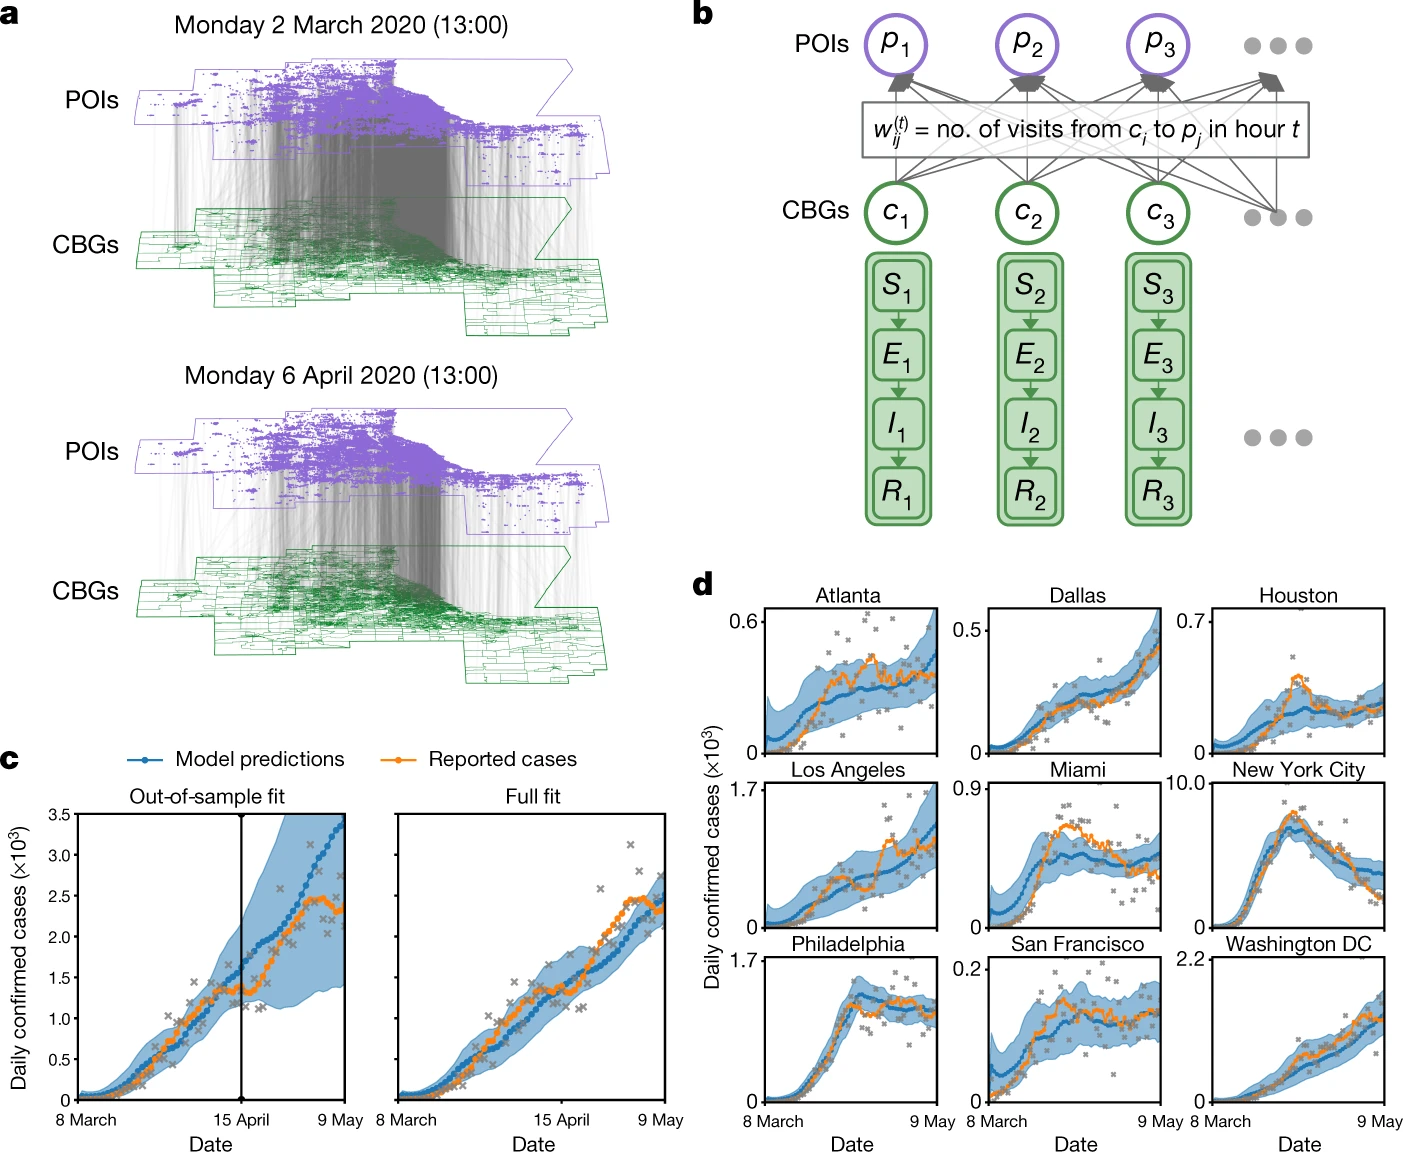
\includegraphics[scale=0.2]{nature-chang-mobility-covid19.png}
        \caption{\gls{SEIR} model informed with mobility data \cite{changMobilityNetworkModels2021}}
        \label{fig:nature-chang-mobility-covid19}
    \end{figure}
\end{frame}

\begin{frame}{Incorporating artificial neural networks}
    \begin{figure}[!htb]
        \centering
        \subcaptionbox{QSIR \cite{dandekarMachineLearningAidedGlobal2020a}}{
            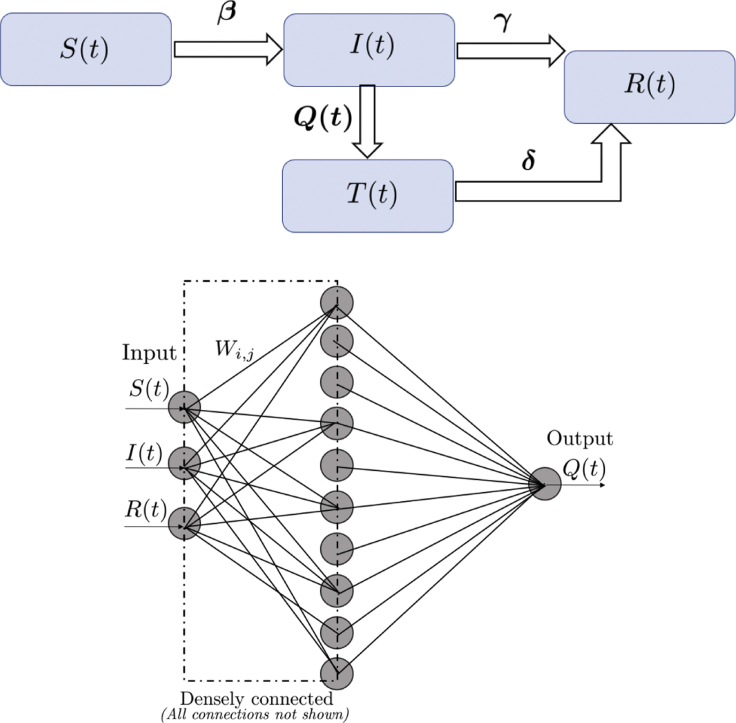
\includegraphics[width=0.4\linewidth]{mit-dandekar-qsir.jpg}
        }
        \subcaptionbox{Time-dependent SIR \cite{jungRealWorldImplicationsRapidly2020}}{
            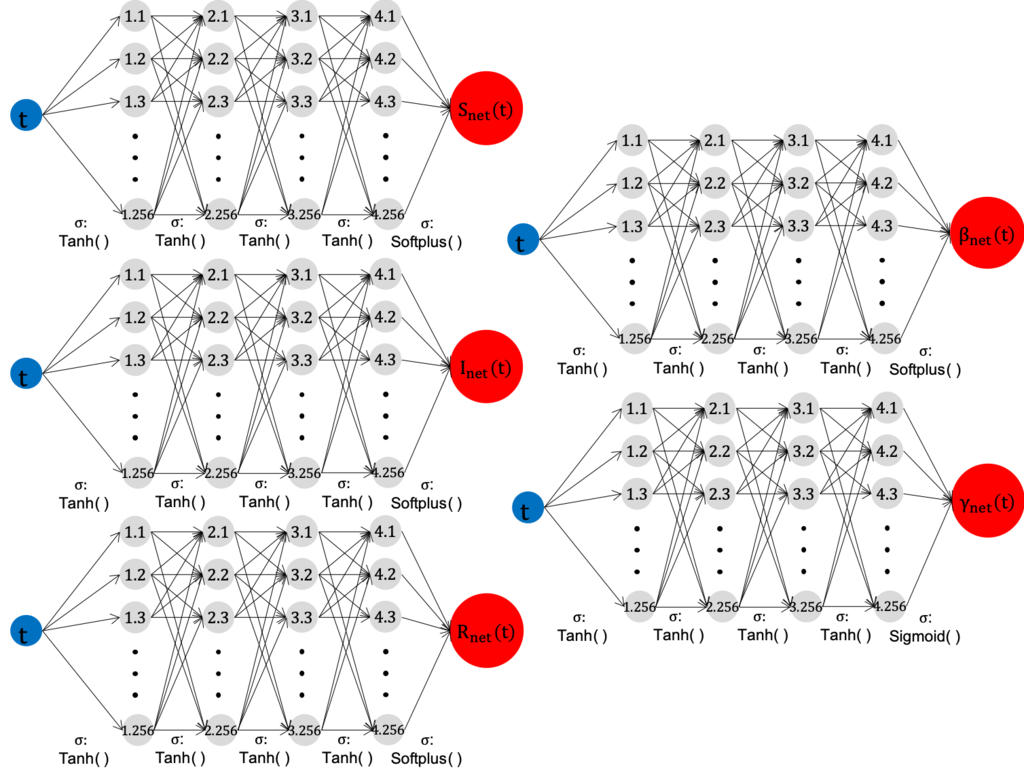
\includegraphics[width=0.4\linewidth]{jung-sir-pinn.png}
        }
        \caption{Predict the parameters of compartmental models with \glspl{ANN}}
        \label{fig:compartmentals-models-with-neural-networks}
    \end{figure}
\end{frame}
